\documentclass[../Book.Stress_regulation.tex]{subfiles}
\graphicspath{{\subfix{../images/}}}
\begin{document}

\section{Definition}

It isn't possible to find a sufficient definition, which describes in a few words what feelings are.\index{feeling}
Generally speaking, it is about the perception of the mental and physical state and the inner movement (= emotion) of a human.

Neurology describes a feeling as the subjective experiencing of excitation and brain--chemical activity.
Love, hate, envy, jealousy, disgust, antipathy, fear, anxiety, sadness, feeling of security, hope are clear designation for the state of a feeling.
Feeling can trigger, reinforce or inhibit actions and increase or numb perception.

\epigraph{Jimmy Carter told me: ``I saw you on TV again on a horse. How come that you look that young?''. I replied to this: ``That's very easy, Jimmy, I'm only taking old horses''.}{\textit{Ronald Reagan}}

\section{A Feeling is Followed by the Emotion}

The media often uses the word ``emotions''.\index{emotion}
It seemingly has a way bigger signification than the word ``feeling''.
People seem to prefer talking about an emotion than talking about a feeling; this last one is often perceived as being more ``intimate''.
This perception is based on some truth: the feeling is the beginning of every emotion.

It's important in this context to clear up the signification of both words: first, we always perceive a feeling.
This feeling in turn causes an emotion.
First and foremost, we should look at how feelings and the reactions caused by them (=emotions) can be changed inside of ourselves.

In this way, we train the instrument that our body is;
an instrument which is able to produce most wonderful melodies, when we're willing to put in the practice to play it properly.
So in the same way that a musician will do their daily finger exercises and continues to develop an ever more intimate relation to his instrument,
in the same way we should invest in the relation to ourselves.
The musician is mastering his instrument, not the other way round.

Stress in all it's form it appears in is in many cases also responsible for feelings and emotions.
A feeling is almost always pleasant or uncomfortable.
That means, we perceive a feeling as positive or negative\index{feeling!positive or negative}.
Situations or people, which provoke pleasant feelings in us tend to attract us.
If people or situations cause uncomfortable feelings, we try to avoid them.

Every human being gets influenced by different things in their lives.
Depending on upbringing, culture, religion and media as well as personal experiences we learned more or less efficiently to express our feelings, to show them or to hide them\index{feelings!hiding}.

\epigraph{Anybody can become angry -- that is easy. But to be angry with the right person and to the right degree and at the right time and for the right purpose, and in the right way -- that is not within everybody's power and is not easy.}{\textit{Aristotle}}


At times, we have a vague ``bad feeling'', but we don't know how to handle it in the concrete situation.
There are also mixed feelings.
For instance with love and pity, the contribution of each of these feelings can be in very different ratios.
A feeling can get so strong that it overwhelms us (tears, anger).
Sometimes we feel afraid of certain feelings in us.
Due to this, we devalue these feelings very strongly.
In situations like these, we perceive ourselves as a plaything of our feelings.

Certain feelings provoke specific reactions, which we control anymore.
Intuitively we notice that we're in a cul-de-sac, in a situation, which seems to have no way out.
Generally we can think clearly, but in certain situations the ever important thinking processes fail us and stop working.
In this manner, we block our own freedom of possible actions and limit ourselves.

At times, we are caught in the discrepancy between our feeling processes and our thinking.
We experience this state as a stalemate.
We're lacking the capacity to make decisions, because both sides, the feelings and the thinking are demanding the fulfillment of their needs.
We lost the thread and any help we had in how to orient.
In these cases, more and more decisions fall by the wayside, which makes us more and more frustrated and unhappy.
When the feelings faded away and we acted according to our patterns of reactions, we only ``become really aware'' of what just happened.
We might get angry at ourselves, because we lost once more our way in a situation like this.
As a matter of fact, we forgot or unlearned to consult on both centers of perception at the time of finding a decision.
But first we have to learn, to get rid of our accumulated ballasts, so that both centers in our brain can start to work again optimally for us.

\section{When Both of Our Brains Aren't Getting Along}

\epigraph{A mind without feelings is inhumane. Feelings without a mind is stupidity.}{\textit{Egon Bahr}}

Both our brains,  \emph{the emotional and the cognitive brain} register\index{brain!emotional}\index{brain!cognitive} the information coming from outside world virtually simultaneously.
After that, they either collaborate well or fight over the control over thinking, feelings and behaviors.
The result of this interaction determines what we feel and how our relation to our surroundings and other people are.
The different forms of rivalry between the two different brains make us unhappy.

\section{What's More Important: Feeling or Thinking?}

\vspace{1cm}

\mytextbox[0]{Translated from~\cite{Berne}
  \vspace{5mm}
   
  \noindent The recipe

  The natural parent--I in the mother and the father is up to a certain degree biologically programmed and has a natural educative and simultaneously a protective character.
  At the very base of it, both parents only want the best for their child.
  They encourage the child in a manner which is meant to bring it success and well--being, according to their world--views and theories of life.
  They transmit it recipes, which they often took over from the grand--parents.
  Examples for the thinking patterns of the middle class are for instance: ``Work hard!'', ``Be a good girl!'', ``Save your money diligently'' and ``Be always on time''.
  At the same times, every family has their own motto, like ``Don't eat any food rich in starch'', ``Never sit down in a public restroom'' or ``masturbation will dry out the spine!''.
}

The cognitive brain controls the conscious attention as well as the skill of dampening the emotional reactions.
This control of the feelings by the cognitive brain avoids a tyranny of the feelings and a life which is completely dominated by instincts and reflexes.

The control of our feelings by the thinking process is a double--edged matter: if it is exerted too often, you might loose the capacity to hear the cries for help of the emotional brain.
People who experienced in their childhood that feelings aren't valid, learned to suppress them.\index{feeling!suppress}
A classical example is: ``Boys don't cry!''.
An exaggerated control of the feelings can lead to insensitivity.

A brain which forbids emotional information to exert an influence also causes other problems.
It will be hard to make decision when you don't have any preferences, no ``inner voices'' which comes from the heart or the belly --- those parts of our body which cause an ``irrational echo''.

\textbf{Goal: A permanent well--being on the base of an inner harmony.
  That's the case, when the emotional and cognitive brain complete each other.
  The emotional brain gives the direction, in which we want to create our life.
  The cognitive brain helps us to go forward in this direction as clever as possible.}

\textbf{Training: Excessively emotional situations can be encountered with cognitive elements and the other way round.}

When a feeling indeed takes the upper hand, it's a advisable to occupy yourself with rational facts.
Just simple arithmetic in your head can have huge effects.
If the cognitive strain is too much we can try to restore the equilibrium with music,
for instance with a slow passage from one of Mozart's pieces (example: Piano concert n. 21, Andante).\index{feeling!regulate}\index{cognitive strain!regulate}


\epigraph{Music expresses that which cannot be put into words and that which cannot remain silent.}{\textit{Victor Hugo}}

\section[Homeostasis]{Homeostasis: I'm Exactly Where I Want to Be in My Life.}

The limbic system\index{system!limbic} in the brain is the control central, which constantly receives information from the diverse body parts and reacts to them,
by controlling physiological equilibrium of the body:
respiration, heart rhythm, blood pressure, appetite, sleep, libido, excretion of hormones, immune system.
The responsibility of the limbic brain is to keep the different functions in a dynamic equilibrium.
Claude Ernanrd, a French researcher and father of modern physiology described that state at the end of the 19th century as \emph{homeostasis}.\index{homeostasis}

\textbf{Homeostasis described the equilibrium between all physiological body function, so the relation of blood pressure, body temperature, body temperature, pH value of the blood, etc.}


From this perspective, our emotions are nothing else but the conscious experiencing of a big interplay of physiological reactions.
They supervise the activity of the biological systems of the our body and adapt those to the needs of the inner and outer surrounding.

The emotional brain knows our body much better than our cognitive brain.
Therefore it is much easier to reach our feelings over our body than over language.
The main emphasis lies on the movement of the body.
Further examples are Gymnastics, Dynamind, Jin Shin Jyutsu, nutrition and acupuncture.\index{emotions!regulating}


Once again: Emotional relations have a strong physical component; we experience them in a physical manner.
That's why this approach to the emotional brain is more direct and efficient than the one over thinking and language.

\vspace{1cm}

\mytextbox[0]{Bruce Lipton, translated from~\cite{LiptonCell}
  \vspace{5mm}
   
  \noindent If you believe, that the genes determine your life and you know, that you have no influence over which genes you received at your conception, then you have all the right in the world to feel as a victim of genetics.
  ``I have no fault that I work so slowly, that I can't keep appointments --- it happens to be my genetic disposition!''

  Since the beginning of the genetic age we have been indoctrinated, that we're under the power of our genes.
  The world is full of people who live in the fear that their genes will one day turn against them.
  How many people live in the fear of being walking time bombs --- they only wait that the cancer will explode into their life, the way it did in the lives of their mother, sister or aunt.

  Millions of people think their fragile health isn't the result of a combination of mental, physical, emotional or spiritual reasons, but attribute it to the insufficient biochemistry of their body.

  Are your kids being naughty?
  More and more parents first reaction is to medication to therapy a ``chemical disequilibrium'',
  instead of taking it on themselves to get to the ground of what is happening in the body, brain and soul of their child.

  There's no doubts that certain diseases, like the Huntington disease, thalassemia major und cystic fibrosis are due to a genetic defect.
  But less than two percent of the population are affected by such diseases.
  By far the bigger part of humanity gets born with genes which would allow them a healthy and happy life.
}

\section{The Power of the Physical Component}

When we're sad, counseling words can express compassion.
More effective and healing on the other hand is a big good hug.
Our language accounts for these bodily reactions with expressions like ``holding the hand'', ``cross your fingers''.
In soccer, the mutual hugs after scoring a goal are legendary.
Lovers feel happy all around, because they permanently communicate on a physical level.
The bigger is the emotional crash, when these physical affections suddenly stop.\index{touch}

\epigraph{The most difficult thing in life is to get the heart and the brain to collaborate. In my case, they are not even on friendly terms.}{\textit{Woody Allen}}

True physical happiness is therefore only possible, when it comes from your heart.\index{brain--heart}
In the animal kingdom you can see how important physical contact is.
For Koalas hugs are the first and foremost survival strategy.
Given that the young Koalas grow up on the back of their bother, hugs are vital for them.
Koalas are very tender with each other and have a well developed social life.
They stay closely connected for their whole life.

Our posture will in most cases expresses our feelings and is able to support a feeling.
When we're standing in a relaxed manner and are in equilibrium, we exactly spend the amount of energy, which is needed to counteract earth's gravity
and which allows us to fully perceive our whole organism.

In this case, we can orient with closed eyes, by totally relying on feeling.
After a while we notice, that the slightest changes in the distribution of the body's weight evokes different sensations of effort or relaxation in the muscle tissue and while breathing.
When we get closer to an equilibrium state, a feeling of lightness, freedom and happiness, which is not comparable to any other sensation.
We discover that we are constantly in a flow; nothing is static.

On a neuro--muscular level is our posture coined by our behavioral habits.
Our posture is the outward manifestation of our feelings: nerves get imprinted by our muscles and the other way around.

\textbf{The essence of a human is something whole. Body and soul penetrate each other to the level, that one of the two always changes with the other one.}

\chapter{Under the Spell of the Feelings}

Feelings develop in an interplay of different components in our body.
The neurotransmitter dopamine reinforces the learning effect from positive experiences.
The early warning system in our brain, the Anterior Cingulate Cortex (ACC)\index{anterior cingulate cortex}\index{system!early warning}
works like a sixth sense and learns to permanently anticipate difficulties and to warn us correspondingly.
The amygdala\index{amygdala} processes feelings.
Even pictures which have been perceived subconsciously will thoroughly influence how feelings are formed.
Fear is localized there.\index{fear}
In the process of learning fear, in two parts of our brain messenger chemicals play an essential role:
The hormone which releases gastrine as well as the neurotransmitter GRP; the gene which is able to dampen fear.

\section{Our Longing for the Always Nice Feelings}


\setlength\epigraphwidth{.7\textwidth}

\epigraph{The warmth \\ \vspace{5mm}
  In spring, kids come to the forest and find a snow man.
  The snow man is crying and contorts his face, because the sun is shining.
  The kids caress him, because they want to help him.
  But their warm hands makes him melt his size even more.

  When are looking for him again later on, they find tender spring blossoms where he was standing.}{\textit{Bert Hellinger}}
\setlength\epigraphwidth{.4\textwidth}

Music is the door to our feelings.
Every person can prescribe themselves their daily dose of feelings.
Our favorite music is capable to to evoke beautiful memories in the different regions of our cerebral cortex.
Music always played an important role in the lives of humans.
By the means of the memory storage i9n our brain, which goes back to the times of our ancestors,
we recorded \emph{rituals and ancient sounds}, which nourish our thinking processes.
All central achievements of society have been accompanied with music.
The ancient musical repertoire of a culture still connects people to their ancestors and gives the security and closeness that we crave.
The healing aspect of music is successfully applied in pain therapy.

When dark feelings and thoughts control a human being, he's prone to fall prey to the fast happiness.
Alcohol is promising fast happiness, at least for a short amount of time.
Most often after  there follows a crash into sadness and depression.

\epigraph{Sorrows don't drown in alcohol. They can swim.}{\textit{Heinz R\"uhmann}}

\section{The Chemical Viscous Circle of Addiction}

The driving force behind the deadly circle of addiction\index{addiction} is pure brain chemistry.
A intricate system of dopamines, gamma--alpha--butyroic acids, peptides resembling opium and serotonin is needed to excrete a feeling of happiness.\index{happiness}
Further information to this topic follows in the module medicine
(Part~\ref{part:medicine} starting on page~\pageref{part:medicine}). % reference to medicine

\section{Crying as the Ideal Painkiller}

Tears\index{crying}\index{tears} are the most obvious signs of our emotional life.
When feelings overwhelm us, crying, but as well laughing give us big relief.
It has an effect of soothing pain, similar to morphine.
Tears, coming form crying or laughing relaxes the muscles and liquefies pain.
With the help of tears, homemade stress can be dissipated.
Tears often often express a wish for fulfillment, closeness or consolation.
Especially in religions, tears are seen as a sign of authenticity and integrity.
After all, crying is an almost exclusively human skill.

But not all tears are alike.
When an object hits an eye or cries while cutting onions, then those are tears due to a stimulus.
They are composed totally differently from the tears spilled over emotions.

\chapter{Feelings vs.  Ratio}

A person who's letting himself being led by his feelings isn't always behaving in an intelligent way.
A term used in this context is the so called ``bipolar dysfunction``.
Feelings have a big hold over our behaviors and at times coax us into actions, which don't necessarily benefit us.

\epigraph{Many people know, that they are unhappy. But even more people don't know, that they are happy.}{\textit{Albert Schweitzer}}

For instance, when a person feels disadvantaged, the bad feelings gain the upper hand.
In this situation, the influence of rational thinking is strongly inhibited.
On the other hand, if a person suppresses their feelings,\index{feelings!suppress} can count on a whole series of heavy health and mental health problems.

And that's not the only effect.
People who control their feelings, can remember emotional experiences significantly less that people who allow their feelings to express.
Every form of control of the feelings will as a consequence influence our perception.

\section{The Power of the Feelings}


Feelings often also have an influence in economic decisions.
Even wall street broker lets his rational decision, when he gets the slightest feeling that he's about to loose money.
So when for instance a bad feeling takes the upper hand, people tend towards relying more on this bad feeling than on their rational thinking.
Even when their decision doesn't bring them any advantages or even makes them suffer bad consequences.

\epigraph{Illnesses do not come upon us out of the blue. They are developed from small daily sins against Nature.
  When enough sins have accumulated, illnesses will suddenly appear.}{\textit{Hippocrates}}

Suppressed feelings\index{feelings!suppressed} can trigger a whole series of heavy health problems and heavily burden the soul.
If we don't want to understand their language, the only way open to get to us is over our boy, given that they indiscriminately mean it well with us.
We have to get sick --- at least as long as we need to start understanding.

\vspace{1cm}

\mytextbox[0]{David Servant--Schreiber, translated from~\cite{MedEmotionen}
  \vspace{5mm}
   
  \noindent \textbf{``Flow state'' and the smile of the Buddha}\index{flow state}\index{smile}

  \vspace{5mm}

  To harmonically live together with other people, it is important to achieve and maintain an equilibrium between our immediate emotional --- instinctive -- reaction and our rational reaction.
  These rational reactions  maintain social bonds over a longer term.
  The emotional intelligence find their expression in the most appropriate way, when both brain systems, the cortical and the limbic system keep collaborating.

  In this state, the thoughts, the decisions and the gestures shape and realize themselves in a  natural way
  and proceed without us having to give it any kind of special attention.
  We know at any time, which choice we have to make and we pursue our goal without any strain in a state of natural focus, given that we act according to our values.
  We constantly strive towards this state of well--being: the visible and complete harmony between the emotional brain,
  which gives us the energy and the direction and the cognitive brain, which regulates the execution.
  
  The great American psychologist Mihaly Csikszentmihalyi, who grew up in Hungary's post--war turmoil dedicated his life to try to understand the nature of well--being.
  He called this state ``Flow''.

  Oddly enough, there is a very simple physiological indication of this harmony of the brains: the smile.
  Already Darwin was researching it's fundamentals more than a century ago.
  A fake smile -- to one you force yourself to for social reasons -- stimulates only the muscles of the cheekbone.
  Those are the muscles which uncover the teeth when you purse your lips.

  In contrast, a genuine smile mobilizes the muscles around the eyes.
  Those muscles aren't able to contract deliberately, by the means of our cognitive brain.
  The order to do so has to come from the primitive, deeper lying limbic domains of our brain.
  That is why eyes never lie: the ripples around our eyes show if a smile is genuine or fake.

  A heart--felt, genuine smile shows us intuitively if our conversation partner is in this moment in a state of harmony, between what he thinks and feels,
  between cognition and emotion.

  The brain has an innate tendency to go towards the ``flow state''. The most universal example is the smile of the Buddha.
  The aim of the natural methods, which I will present in the following chapters is to allow this to happen.
  In contrast to the IQ, which barely develops to a higher level during our life time, the emotional intelligence can be cultivated and developed at any age.
  It's never too late to learn, how to better deal with your feelings and your relation to other people.

  The first approach described here is without any doubts the most fundamental one.
  It's about optimizing the heart rhythm, in order to withstand the stress, to get the anxiety under control and to maximize our innate vitality.
  This is the first key to the emotional intelligence.
}

\section[Bodily Processes and Emotions]{Bodily Processes and Emotions are Highly Correlated}

The killer cells of the immune system are the first defensive line of the organism.
As most of our bodily functions, the activity of the killer cells is also regulated by our emotional brain.\index{emotions--body correlation}
Positive feelings like calmth and well--being activates them, while fear, stress and depression inhibits their activity.

\epigraph{I think you are unhappy, because you  never were unhappy. You strode through life without ever facing adversity.
  Nobody knows what you are capable of, not even yourself.}{\textit{Lucius Annaeus Seneca}}

It is impossible to make no painful experiences in life.
If a ``bad'' experience was eventually really bad and if we want to learn from it something for our life, that is totally up to ourselves.

It's desirable to recognize the own potential and to unfold it.
The fear which might flame up during the first steps in a new direction are old acquaintances.
Out of that reason, we should include them into our lives as helpers: whenever I feel at unease, I know that something isn't in order.

Fears have this wonderful trait, that they dissolve into thin air, when you \emph{meet them on eye level}.\index{fears}
They actually want that we do that again and again.
Looking at it this way, it is a marvelous thing.
We are never alone and have a marvelous navigation system in our brain, which knows everything that we are supposed to know.
When the feelings gets too often sacrificed to the ratio, it will take revenge on totally different places.
We fall that much easier for emotional bait (commercials, entertainment industry, political activities).

\section{Self--Handicapping: Good or Bad?}

\vspace{1cm}

\mytextbox[0]{from Zimbardo, Psychologie~\cite{ZimbardoPsych}
  \vspace{5mm}
   
  \noindent One of the main assumptions of the research into the concept of self is that people try to determine themselves clearly,
  because they are searching for a coherent\footnote{coherent: connected, interrelated} identity definition of themselves.
  The age of youth the middle age of being an adult are times of intense search, caused by the fact that a lot is changing or gets questioned.
  Big parts of social psychology are based on the idea, that people want to have exact information about their surroundings and their own place in this world.

  Surprisingly, a few of the interesting current research showed that people are actually doing the opposite.
  For instance, people who are suffering from anxious insecurities and doubts about themselves can only keep up their sense of their own competence,
  if they avoid a decisive check of their own competence.
  There is an irony in this that the advantages of avoiding a check of their competence are weighted heavier than the advantages of a clear, meticulous and exact self--assessment.
  The phenomena of self--handicapping gives us a good illustration of this.

  During self--handicapping\index{self--handicapping}, the goal of the person who's doubting himself is to minimize the influence of the own capacities (more exact: the lack of own capacities) as plausible
  explanation for bad performance.
  We are living in a world in which a big part of what we do will get judged by ourselves and others, with the focus on the competences which are at the base of the observable behavior.

  The performance on the tennis court, in the class room, at work and in society is meticulously judged to determine the athletic, intellectual, artistic or social competence.
  But what happens, if that person to be judged has a handicap --- a broken tennis racket, a heavy cold, a sleepless night or a clammed up conversation partner?
  Isn't it in this case unfair to see failure as an expression of the self?
  A person who handicaps themselves follows this logic --- he/she erects a barrier on the path to successful actions.

  Self-handicapping is, expressed briefly, ``a reaction to an anticipated loss of self--respect''.\index{self--respect!protection}
  It is therefore a phenomena which can be classified under the time--honored motive to protect the self--respect or the perceived value of yourself.

  A person who is putting themselves at an disadvantage must have an endangered and fragile, but not a totally negative concept of self.
  An eternal looser who has no or little self--respect after a long and painful history of inadequacies isn't the candidate for self--handicapping.
  A decisive basis for the strategy of self--handicapping is that the person has something to protect.

  If you're assuming, that many different behaviors can be signs of self--handicapping, then you're on the right track.
  An overview over 3 dozen studies which exist to this topic since 1978 reports cases of pusillanimity\footnote{tendency to hesitate, out of a tendency towards anxiety.},
  laziness, abuse of drugs and alcohol\index{abuse!substance}\index{abuse!alcohol}, moodiness, attempting the impossible and many other incarnation of self--handicapping in daily life.
  Even though self--handicapping aren't as widespread as the search of an understanding of the self,
  it nevertheless seems to be clear, that humans often prefer ambiguity over clarity of themselves ---
  especially when that clarity could be not that charming.
}

\chapter{The Healing Power of Laughing}

The laughing muscles are pressing on a nerve and this nerve transmits signals to the brain, which in turn realizes that their human is smiling.\index{laughing}\index{smile}
Caused bu this reaction, the brain excretes ``joy hormones'', the so called \emph{endorphins}.\index{endorphins}

The saying goes, that ``laughing is the best medicine''.
This wisdom got scientifically confirmed by laughter researcher, the so called gelotologists (Greek gelos = laughing).
Gelotology\index{gelotology} is concerned with the physical and psychological effects on humans of laughing and smiling.
A humorous event, which seduces us to laugh or at least smile, is called an exhilaration.
This can be triggered by a plethora of unrelated stimuli.

\epigraph{Humor is the umbrella of the wise ones.}{\textit{Erich K\"astner}}

Already Aristotle\index{Aristotle} (Greek philosopher) and Cicero\index{Cicero}
(Roman politician, writer and speaker and mediator in the sense of Greek education) were researching the sources of humor.
They were attributing laughing to the perception of defects of a human which was perceived as inferior (degradation theory).\index{degradation theory}
Each comedy is constructed by this pattern.
The beginning of clowns and jesters are based on this.

Research of laughter became popular at the end of the 70ies, when the science journalist Norman Cousin\index{Norman Cousin} laid the decisive foundation with the report of his experiences.
The doctors gave him a very unfavorable prognosis as Cousin was suffering from a severe and very painful inflammation of the spine.
He  knew about the negative effects of a pessimistic attitude on the progression of diseases.
He changed the hospital room up into a hotel room.
He was consciously consuming funny movies and humorous books, to systematically get himself laughing.
Thereby he made a fantastic discovery: after ten minutes of intense laughing, his pains subsided and he was able to sleep for two hours without problems.
Cousin completely recovered, even though nobody could really explain why.

\section{Laughing is Balm for the Body and the Soul}

Laughing has a pain--relieving effect and strengthens the immune system.\index{immune system}\index{laughing!effects}
For instance are the values of the natural killer cells and antibodies higher in people, who just have seen a funny movie.
Japanese researcher were able to treat this way successfully allergies, by amusing the patients with movies.

\epigraph{There's a fool--proof way to distinguish between truly great men and the ones which only seem great: All great men have a sense of humor.}{\textit{Ludwig Reiners}}

Laughing is almost like internal jogging: we activate up to 80 muscles, when we're laughing out loud.
This has also a positive effect on the heart--circulation system.
We breathe more intensely and deeply from our belly.
The lung gets well oxygenated, which leads to higher oxygen levels in the blood.
This in turn activates the combustion processes in the body.
First, the heart rate increases, and soon after decreases again, which leads to a decrease of our blood pressure.
The muscles, which were tensed up as we started laughing, relax in a sustainable manner.

Laughing also lowers the production of the stress hormones adrenaline and cortisol.
Instead, the body excretes endorphin.
In hospitals clowns are officially working in the sense of the happiness hormones.

\textbf{A minute of heart--felt laughing is as refreshing as 45 minutes of relaxation training.}

The list of positive effects of laughing is almost endless.
According to gelotologists, laughing also inspires creativity.
The craziest and most entertaining ideas are often born when the meeting degenerated into good-humored silliness.
At least very impressive and extraordinary commercials often got created in this manner.

Truly a means for everything!
Laughing keeps us fit, helps against spring exhaustion and furthermore increases the sexual performance.
Regardless of all these successes, the modern psychotherapy still meets humor with a certain skeptical attitude.

Imagine laughing would be the only thing by which we let ourselves be infected by!

Regardless of the incredible power of laughter, we tend to loose that capacity more and more.
The statistic shows clearly: \emph{While kids laugh up to 400 times during a day, adults only laugh about 15 times a day.}

A few hints, how we can bring it back up to 400 times a day:
\begin{itemize}
\item Even a smile is already enough.
\item Listen to laugh CDs.
\item Look for really funny comic strips in the internet and share them with others.
\end{itemize}

\vspace{1cm}

\mytextbox[0]{Roland Schutzbach and his partner Christine about laughing~\cite{Lachen}
  \vspace{5mm}
   
  \noindent ``We are so happy and cheerful and laugh the whole time''.
  It is called laughing as a habit: laughing became internalized,
  ``and when something goes wrong, we start by laughing about it and then as a second action, we prefer to stop it''.
  
  Many communities still have this old, ``problem oriented'' trait, which signifies:
  ``We have to rescue the world and we have to help the others and we are so important''.
  For the 'foolosophe' it is very clear, that ``they take themselves to be way too important.''
  And exactly that is the main insight from laughing, that ``nothing is really important, the least of all me''.
  The most important things always have been here and always will be be here.
  
  \noindent www.patchadams.org,

  \noindent www.laughteryoga.org,

  \noindent www.wakeuplaughing.com, 
}

\chapter{Definitions: The Emotion}
\section{Classification of Emotions}
% Here is the gap p 23 & 24

Older theories put the feelings into four main categories: fear, anger, joy and sadness.

\epigraph{There's nothing more silent than a loaded cannon.}{\textit{Heinrich Heine}}

Another system of classification is to distinguish between feelings and affects.\index{affect}
According to this way of classifying emotions, feelings are the emotions which unite us, and affects are emotions which separate us.
in the category of feelings would then be: love, friendship, compassion, connection and feeling of community.
Under affects go: envy, hate, fear, jealousy, inferiority feeling and a feeling of guilt.

Studies of different cultures showed, that feelings aren't necessarily identical with the shown emotion.
Cultural factors influence the observable expression of emotions in contrast to the inner, felt reality of the feeling,
how a feeling is individually experienced in their inner world.

In each culture exists many basic emotions.\index{emotion!basic}
They are closely linked to the simultaneously occurring neuronal processes.
Nowadays the assumption is made, that the fundamental emotions are in a narrow connection with the corresponding facial expression.
In a study across many different cultures has for instance always attributed anger to lowering and contracting the eye brows,
pulling the eyes into slits and squeezing the mouth together.
The mimic expression of a basic emotion is looked at as being universal.

\section{Ways to Regulate Emotions}

Emotions often get triggered by situations, people, places or memories and often are focus on a specific object.\index{emotions!regulate}
A certain person can trigger wonderful joy, or then debilitating fear.
Cognition's like music, smells or pictures can also trigger feelings or change them.
For instance, smells often trigger memories of past feelings.
Emotions are get triggered very quickly or then build themselves up slowly.
They are not able to be directly influenced.
But we can learn, how to deal with our emotions.

\epigraph{An eye for an eye will only leave the whole world blind.}{\textit{Mahatma Gandhi}}

Our behavior has a certain feedback on our feelings.
In this sense, there are 3 ways for regulation open to us:
We can reinforce our emotions through thoughts and actions,
slowly changing them up
or let them slowly subside.
On a physical level are for instance \emph{meditative exercises, sleep, hunger, feeling of being full, being tense, jogging or yoga} influencing our emotions.

Emotions have a strong influence on the performance of a human, without a doubt.
In this sense, the so--called \emph{emotional intelligence}\index{intelligence!emotional} gets more and more in the focus of our interests.
The validity of the construct ``emotional intelligence'' is nevertheless still very much controversial in
empirical\footnote{empirical: coming from experience, observations and the experiment.} psychology.

\section{The Physiology of the Conflict Scale}

An animal has to be in a state of high action potential in case of imminent danger.\index{action potential}
A vegetative chain reaction gets triggered by the excretion of adrenaline by the adrenals in order to provide the energy necessary.
This leads in turn to an increase in blood pressure, and blood sugar levels and the tension in the muscles.

The aim is to provide a maximum amount of energy for survival.
This inherited stress reaction is causing most stress problems for modern humans.
We're pretty much all the time on the flight from the tiger.
Thai means, we're trapped constantly in a trigger--reaction scheme, into which there's a permanent input of too many stimuli, without the vital breaks.
We often have not enough possibility of arranging things ourselves.
The inner level of tension is constantly being increased and we perceive that as uncomfortable, as a prison of stress.\index{tension}

With our biological configuration we react the same way as our ancestors in the Savannah.
The exterior world has changed, became more complex and more confusing in it's layout.
Surprising escalation of violence, completely out of balance, as they appear more and more often seem to be a consequence of the biological mechanisms.
These escalations of violence seem to be triggered by the perception of existential threats.\index{anger reaction}

In this context, the similarity of a stimulus with an earlier experienced situation is decisive for the initial triggering of these archaic reactions.
A real existing danger is not at all decisive.
People get more and more often in a state of emergency, let themselves being carried away to outbreaks of anger and violent actions,
without the cognitive brain having a chance to examine these actions in more detail.\index{viscous circle!anger reaction}

\epigraph{A sensitive person is a person who, because they have corns himself, always treads on other people's toes.}{\textit{Oscar Wilde}}

The more or less fast escalation of rage and anger in situations of conflict is way more often to be observed  than the above mentioned instantaneous derailment of the emotions.
This process is also able to be explained on a physiological level.
By angry or hostile reactions to an event will the limbic system be put in a state of excitation through the excretion of certain chemicals.
This state continues hours after the original events which triggered that state ended.
In this time, the threshold for a next anger reaction is lowered.

For instance the irritated atmosphere after a day at work with a lot of anger continues and is able to to trigger us to get angry in an immoderate way
over the driver in front of us in traffic or a fly on the wall.
If acute anger reactions follow, more stress hormones get released.
The excitation level of the limbic system continues to increase in this manner.
Given that these reactions Durer for a while, the effects overlap.
Anger escalates due to the lowered tolerance threshold faster and faster, up to the point where the emotional brain declares a state of emergency.
That way, a latent elevated adrenaline level gets maintained in our body, and frustration and depression is then not far.

People who mismanage themselves over an extended period of time, more and more withdraw in their own snail shell.
The fears of change then grow higher and higher around that snail shell.
The affected person then fears loosing himself, and collapsing.
Nobody wants to volunteer loosing face.
But many people afflicted by that fear don't realize that they are unable to loose face, but just a mask.\index{loosing face}
And even more a mask which isn't even fitting to them in the first place.
Behind that, the \emph{freedom} is growing.
The goal is to reach equilibrium; in this case by \emph{taming the emotions}.

\vspace{1cm}

\mytextbox[0]{Translated from Bert Hellinger
  \vspace{5mm}
   
  \noindent The clearing
  \vspace{5mm}

  Somebody lives in a little house and during the years a lot of clutter accumulates in the rooms.
  Many guests brought their things, and when they push along they left many suitcases there in the little house.
  It's almost as if they are still there, even if they left a a long while ago.

  The owner also accumulated things and those things stayed in the house.
  Nothing should be over or get lost.
  Memories are also attached to broken things, so they stay and take the space away from better things.

  Only when the owner almost asphyxiates, he starts to clean up.
  He starts with his books.
  Does he still want to look at the old pictures and understand the lessons and stories of others?
  He gets out of his house, what is worked off a long time ago and in his rooms it gets bright and airy once again.

  Then he starts opening suitcases of others and looks if he can find something which he still can put to use.
  Thereby he discovers a few valuable things and put them aside.
  The rest he gets out of the house.

  He throws the old stuff in a deep ditch, carefully covers it with soil and then he sows grass over it.
}

\chapter{The Heart--Brain System}

The so--called peripheral autonomous (vegetative) part of the nervous system\index{nervous system!autonomous!peripheral} is the closest connection
between the semi--autonomous neuronal networks of the small brain of the heart\index{heart!brain} and the emotional brain.
This connection manages the operations of our organs, but totally eludes our will and awareness.
The heart and our emotional brain interact and influence each others.
They build a veritable heart--brain system.\index{nervous system!autonomous}

The \emph{autonomous nervous system}\index{nervous system!autonomous} has a very importance position.
It consists of two strands which originate in the emotional brain and stimulate all organs of the body.
The one strand, called the sympathetic\footnote{The expression ``sympathetic'' has a Latin roots and means ``to be in connection''.
  The nerves of sympathetic nervous system are connected with the spine all along the whole spinal column.} nerve,\index{nerve!sympathetic} 
releases adrenaline and noradrenaline and regulates the fight and flight\index{reaction!fight and flight} reactions.
He increases the heart rate and activates the emotional brain.
The other strand of the autonomous nervous system is the antagonist of the sympathetic nerve and is therefore called the parasympathetic nerve.\index{nerve!parasympathetic}
It releases the neuro transmitter acetylcholine\index{acetylcholine}, which is active in relation with the states of relaxation.
Acetylcholine decreases the heart rate.

The interplay of these two ssytems can be compared with the \emph{gas pedal} and the \emph{brakes}.
In mammals, these two systems are constantly in equilibrium.
This advantage allows them to adapt extremely fast to changes in their environnment.
For instance a rabbit eating herbs in front of his burrow can stop for a moment, put their ears up, listens and sniffles to detect a potential predator.
Is there no sign of danger, it immediately returns to it's meal.
Only mammals have this adaptation.

        \begin{figure}[htb!]
          \centering
          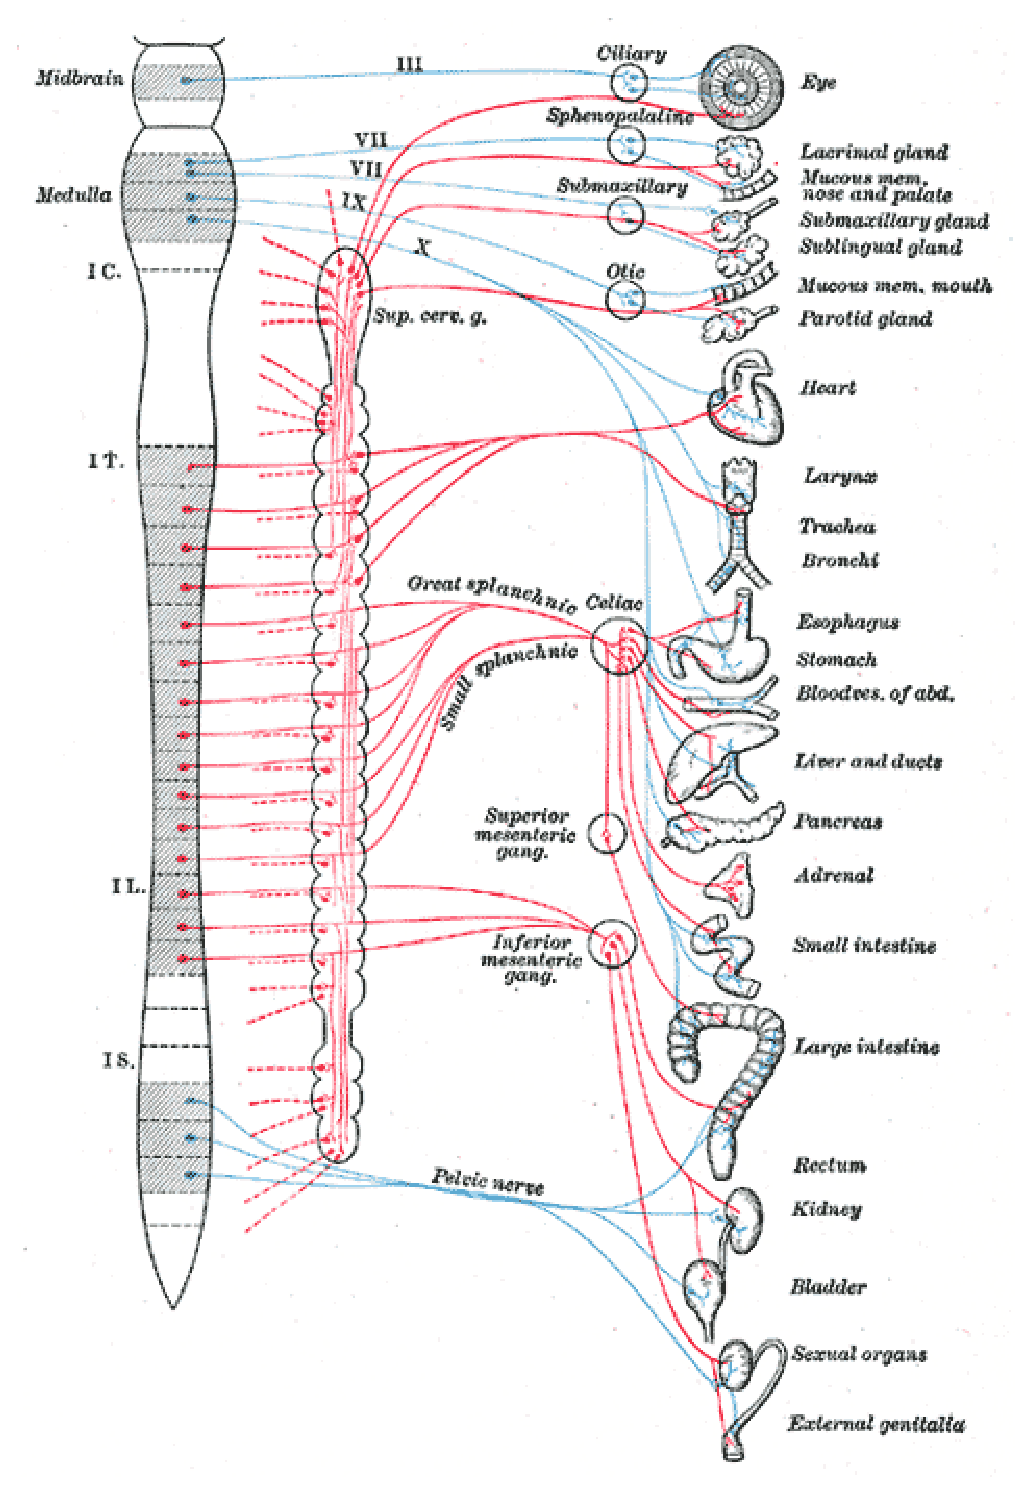
\includegraphics[width=12cm]{AutonomousNS}
          \caption{The autonomous nervous system:
            Diagram of efferent sympathetic (red) and parasympathetic (blue) nervous system.~\cite{LeaAnatomy} over~\cite{Bartleby}}\label{pic:AutonomouNS}
        \end{figure}
        
\chapter{The Area of Influence of the Emotional Brain}

All beings who are equipped with a central nervous system have an emotional brain\index{brain!emotional} with it's seat in the limbic system.
During evolution, the cortex and the neocortex (the ``thinking'' brain) start to show up, humans found their upright gait and conscious processes of thinking got bootstrapped.

\end{document}